\documentclass[letterpaper]{article}
\usepackage[utf8]{inputenc}
\usepackage[spanish]{babel}
\usepackage[letterpaper,includeheadfoot, top=.5cm, bottom=3.0cm, right=2.0cm, left=2.0cm]{geometry}
\renewcommand{\familydefault}{\sfdefault}
\usepackage{amsmath}
\usepackage{graphicx}
\usepackage{subcaption}
\usepackage{gensymb}
\usepackage{color}
\usepackage{hyperref}
\usepackage{amssymb}
\usepackage{url}
%\usepackage{pdfpages}
\usepackage{fancyhdr}
\usepackage{enumerate}
\usepackage{enumitem}
\usepackage{float}
\usepackage{tikz}
\usetikzlibrary{patterns}
\usepackage{siunitx}
\usepackage{framed}
\tikzset{
every picture/.append style={
  execute at begin picture={\deactivatequoting},
  execute at end picture={\activatequoting}
  }
}
%-------------------- CABECERA ---------------------
\pagestyle{fancy}
\fancyhf{}
\author{Docente: Martin}
\date{}
\title{\bf Guía 15: Torque y Estática}
%Encabezado
\fancyhead[R]{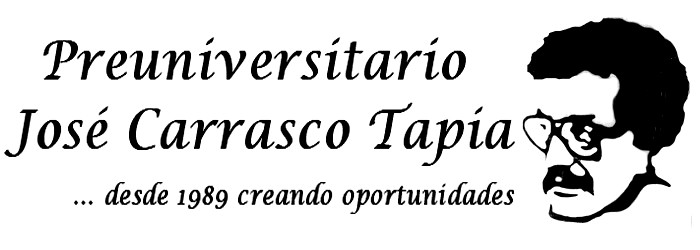
\includegraphics[scale=0.35]{jct.jpg}}
\fancyfoot[C]{\thepage}


\newcommand{\tpb}[1]{node[midway, below, sloped] {#1}}
\newcommand{\tpa}[1]{node[midway, above, sloped] {#1}}
\newcommand{\tvec}[3]{[->, thick] #1 -- #2 \tpb{#3}}
\newcommand{\tveca}[3]{[->, thick] #1 -- #2 \tpa{#3}}
\newcommand{\tvecnotsloped}[3]{[->, thick] #1 -- #2 {node[midway, above] {#3}}}

\newcounter{propiedades}
\newcounter{definiciones}

\newcommand{\propi}{\stepcounter{propiedades} \textbf{Propiedad \thepropiedades}: }
\newcommand{\defii}{\stepcounter{definiciones} \textbf{Definición \thedefiniciones}: }

\newenvironment{prop}
{ \begin{framed} \propi}
{ \end{framed} }
\newenvironment{defi}{\begin{framed} \defii}{\end{framed}}

\newenvironment{enumalf}
{\begin{enumerate}[label=\Alph*)]}
{\end{enumerate}}
\newenvironment{enumroman}
{\begin{enumerate}[label=\Roman*)]}
{\end{enumerate}}

\renewcommand{\sectionmark}[1]{\markright{\thesection.\ #1}}
\renewcommand{\headrulewidth}{0.5pt}
\renewcommand{\footrulewidth}{0pt}
\setlength{\headheight}{92pt}

% --------------- ---------PORTADA -----------------------
\begin{document}
\maketitle
\thispagestyle{fancy}
\begin{center}
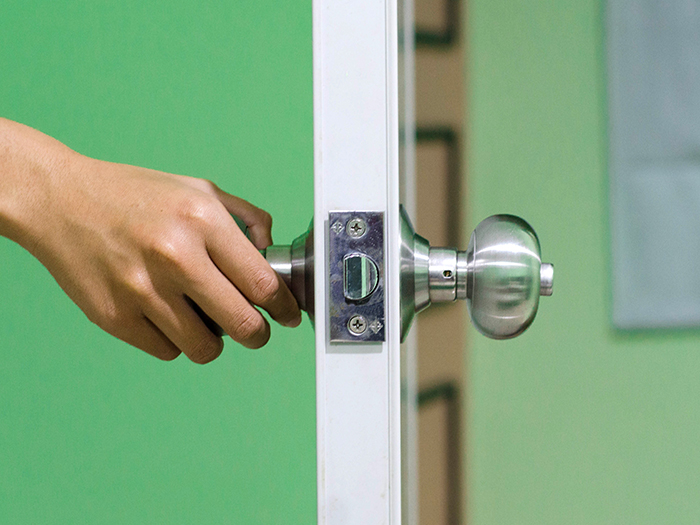
\includegraphics[scale=1.2]{portada.jpg}
\end{center}
\pagebreak

¿Por qué el pomo de la puerta está del lado opuesto a las bisagras? ¿Qué cambiaría si uno pone el pomo de la puerta del lado de las bisagras? ¿Por qué no se puede balancear un lápiz sobre su punta? Aunque estas preguntas puedan parecer muy estúpidas, la respuesta no es trivial. Todo esto y mucho más lo resolveremos al final de esta guía!

\section*{Introducción}

Hemos aprendido que las fuerzas provocan cambios en el movimiento de los objetos a través de $F = ma$. Sin embargo, esto solo explica la traslación de los objetos que constituye solo una parte del movimiento de los cuerpos. Un ejemplo se presenta cuando lanzamos una botella plástica esperando que caiga de verticalmente y quede estable, procediendo después a hacer un \emph{dab}. Ahí la botella no solo se traslada de nuestra mano hasta el piso (de lo contrario sería demasiado fácil y no se merecería un \emph{dab}), sino que también rota en el aire. Pero, ¿por qué se produce esa rotación?

Como veremos a lo largo de esta guía, esa rotación se debe a que ejercemos una fuerza sobre el cuerpo, esa fuerza provoca un torque en el cuerpo y el torque se traduce en movimiento rotacional.

\section*{¿Cómo se define el torque?}

Antes de definir el torque tenemos que entender unos conceptos primero. Al momento de abrir una puerta, uno puede comprobar experimentalmente dos cosas: 
\begin{itemize}

\item es más fácil abrirla mientras más lejos del eje de rotación (donde están las bisagras) la empujemos.

\item es más fácil abrirla mientras el ángulo entre la dirección de la fuerza y la puerta se acerca a \ang{90}.

\end{itemize}

Podemos entonces deducir que antes de definir el torque tenemos que definir esta distancia entre el eje de rotación y el punto donde se aplica la fuerza, y el ángulo. Para esto es muy útil pensar en el vector que va desde el eje de rotación hasta el punto donde se aplica la fuerza. A este vector se le llama brazo de palanca.

\begin{defi}
El brazo de palanca se suele escribir como $\vec{r}$ o $\vec{b}$ y representa el vector que va desde el eje de rotación hasta el punto donde se aplica la fuerza.
\end{defi}

Volviendo al ejemplo de la puerta, podemos pensar en el caso que aplicamos dos fuerzas en distintos puntos y con distinta dirección, como en la figura siguiente. El problema es, ¿qué fuerza permite abrir con mayor fácilidad la puerta? La respuesta está en el torque.

\begin{figure}[h]
\centering
\begin{tikzpicture}
\fill [pattern=north east lines] (0,0) rectangle (5,0.5);
\draw (0,0) rectangle (5,0.5);
\draw [->] (4.5,0) -- (6,2) node[midway, below, right] {$\vec{F}_2$};
%\draw (4.5,2.5) node[above] {$\vec{F}_2$};
\draw [->] (0,-0.6) -- (4.5,-0.6) node[midway, below] {$\vec{r}_2$}; 
\draw [->] (3.5,0) -- (3.5,2.5);
\draw (3.5,2.5) node[above] {$\vec{F}_1$};
\draw [->] (0, -0.1) -- (3.5, -0.1) node[midway, below] {$\vec{r}_1$};
\end{tikzpicture}
\end{figure}

\begin{defi}
El torque o momento de fuerza es un vector que se define como el producto cruz entre el brazo de palanca $\vec{r}$ y la fuerza aplicada $\vec{F}$,
$$\vec{\tau} = \vec{r}\times\vec{F}$$

Lo que es equivalente a,
$$|\vec{\tau}| = |\vec{r}|\cdot|\vec{F}|\cdot\cos{\theta}$$

Donde $\theta$ representa el ángulo que se forma entre la fuerza aplicada y el brazo de palanca, y la dirección de $\vec{\tau}$ está dada por la regla de la mano derecha.

Se deduce que la magnitud del torque se mide en \si{N.m}
\end{defi}

Volviendo al ejemplo de la puerta, tomemos $r_1 = 0.4\ \si{m}$, $F_1 = 10\ \si{N}$, $\theta_1 = \frac\pi2\ \si{rad}$, $r_2 = 0.8\ \si{m}$, $F_2 = 10\ \si{N}$ y $\theta_2 = \frac\pi3\ \si{rad}$, donde $\theta_2$ representa el ángulo entre $\vec{r}_2$ y $\vec{F}_2$. ¿Qué fuerza ejerce un mayor torque?

Primero, notemos que por la regla de la mano derecha, $\vec{\tau}_1$ y $\vec{\tau}_2$ tienen la misma dirección y sentido, basta entonces ver qué vector tiene mayor magnitud. Luego, aplicamos la definición de torque:
\begin{align*}
|\vec{\tau}_1| &= |\vec{r}_1|\cdot|\vec{F}_1|\cdot\cos{\theta_1} = 0.4 \cdot 10 \cdot \cos{\frac\pi2} = 4\ \si{N.m} \\
|\vec{\tau}_2| &= |\vec{r}_2|\cdot|\vec{F}_2|\cdot\cos{\theta_2} = 0.8 \cdot 10 \cdot \cos{\frac\pi3} = 8\cdot\frac12 = 4\ \si{N.m}
\end{align*}

Sorprendentemete, las dos fuerzas producen el mismo torque! ¿Pero qué significa eso respecto al movimiento de la puerta? Para responder a esta pregunta tenemos que introducir una relación muy importante para el estudio de la rotación de los objetos, la famosa segunda ley de Newton para la rotación:

\begin{prop}
El torque y la aceleración angular están íntimamente relacionados de manera análoga a la fuerza y la aceleración lineal:
$$\vec{\tau} = I\vec{\alpha}$$

Donde $I$ representa el momento de inercia de un cuerpo y $\vec{\alpha}$ su aceleración angular.
\end{prop}

\section*{Equilibrio estático}

Un problema recurrente en el estudio de fuerzas y rotación, son las condiciones para que un cuerpo esté estático. Se entiende que un cuerpo está estático cuando está y permanece en reposo. En otras palabras, su aceleración y su velocidad son nulas. De manera formal, para que un cuerpo esté completamente estático se tienen que cumplir cuatro condiciones:
\begin{itemize}
\item La velocidad lineal $v$ tiene que ser nula.
\item La fuerza neta sobre el objeto tiene que ser nula.
\item La velocidad angular $\omega$ tiene que ser nula.
\item El torque neto sobre el objeto tiene que ser nulo.
\end{itemize}

Es importante notar que incluso si la fuerza neta sobre un cuerpo es nula, eso no implica que el torque neto sea nulo. Dos fuerzas de igual magnitud que tienen sentido opuesto pero se aplican en distintos puntos del cuerpo provocan un torque neto que no es nulo mientras que la fuerza neta sobre el cuerpo si es nula. En particular, en la figura siguiente vemos que:

$$\sum\vec{F} = \vec{F}_1 + \vec{F}_2 = 0$$

Mientras que si analizamos el torque sobre el cuerpo, veremos que $\vec{\tau}_1 = \vec{r}_1\times\vec{F}_1$, aplicando la regla de la mano derecha tendremos que $\vec{\tau}_1$ tendrá sentido negativo al igual que $\vec{\tau}_2$. De ahí que $\vec{\tau}_1 = -|\vec{r}_1|\cdot|\vec{F}_1|\cdot\cos{\theta_1} = -F_1\cdot r_1$ y $\vec{\tau}_2 = -|\vec{r}_2|\cdot|\vec{F}_1|\cdot\cos{\theta_2} = -F_2\cdot r_2$. Donde $F_1$, $r_1$, $F_2$, $r_2$ son las magnitudes respectivas de los vectores $\vec{F}_1$, $\vec{r}_1$, $\vec{F}_2$, $\vec{r}_2$. Para simplificar el ejemplo, digamos que $F_1 = 
F_2$ y $r_1 = r_2$. Finalmente,

$$\sum\vec{\tau} = \vec{\tau}_1 + \vec{\tau}_2 = -F_1\cdot r_1 - F_2\cdot r_2 = -2F_1\cdot r_1 \neq 0$$

Podemos concluir entonces que la suma de fuerzas o la fuerza neta será nula, lo que se traduce en equilibrio traslacional (el objeto no se traslada). Sin embargo, la suma de torques o el torque neto no será nulo, por lo tanto, el objeto rotará, \textbf{no} estará en equilibrio rotacional y tampoco estará completamente estático.

\begin{figure}[h]
\centering
\begin{tikzpicture}
\fill [pattern=north east lines] (0,0) rectangle (4,2);
\draw (0,0) rectangle (4,2);
\draw [->] (1,0) -- (1,1.5);
\draw (1,0) node[below] {$\vec{F}_1$};
\draw [->] (2,-0.1) -- (1,-0.1) node[midway, below] {$r_1$};
\draw [->] (3,2) -- (3,0.5);
\draw (3,2) node[above] {$\vec{F}_2$};
\draw [->] (2,2.1) -- (3,2.1) node[midway, above] {$r_2$};
\end{tikzpicture}
\end{figure}
 
\section*{Ejercicios}

\begin{enumerate}

\item La condición para que una puerta gire en torno a un eje es que se aplique

\begin{enumerate}[label=\Alph*)]
\item un impulso sobre ella.
\item un torque sobre ella.
\item una fuerza sobre ella.
\item una fuerza en el eje de giro.
\item ninguna de las anteriores
\end{enumerate}

\item La puerta giratoria de un edificio en cierto instante queda detenida debido a la acción de las cargas que indica la figura. ¿A qué distancia se aplicó la carga $\frac{P}{2}$

\begin{figure}[h]
\centering
\begin{tikzpicture}
\draw (0,0) rectangle (4,1);
\draw (2,0.5) node {$\bullet$};
\draw [<->] (0.2,-0.2) -- (1.8,-0.2) node[midway, below] {$x$};
\draw [<->] (2.2,-0.2) -- (3.8,-0.2) node[midway, below] {$4L$};
\draw [->] (0,4) -- (0,1.3);
\draw (0,4) node[above] {$\frac{P}{2}$};
\draw [->] (4,4) -- (4,1.3);
\draw (4,4) node[above] {$P$};
\end{tikzpicture}
\end{figure}

\begin{enumalf}
\item $L$
\item $2L$
\item $4L$
\item $6L$
\item $8L$
\end{enumalf}

\pagebreak

\item En la figura siguiente, determine la magnitud del torque neto y el tipo de giro (horario o antihorario). Considere $|\vec{F}_1| = 3\ \si{N}$, $|\vec{F}_2| = 7\ \si{N}$, $|\vec{F}_3| = 5\ \si{N}$.

\begin{figure}[h]
\centering
\begin{tikzpicture}
\fill (0,0) -- (1,0) -- (0.5,0.7) -- cycle;
\draw (0.4,0.7) rectangle (4.5, 1.3);
\draw [->] (1.7,1.3) -- (1.7,2.3);
\draw (1.7,2.3) node[above] {$\vec{F}_1$};
\draw [<->] (0.5,1.5) -- (1.5,1.5) node[midway,above] {$2\ \si{m}$};
\draw [<->] (1.9,1.5) -- (2.9,1.5) node[midway,above] {$2\ \si{m}$};
\draw [<->] (3.3,1.5) -- (4.3,1.5) node[midway,above] {$2\ \si{m}$};
\draw [->] (3.1,0.7) -- (3.1, -0.3);
\draw (3.1,-0.3) node[below] {$\vec{F}_2$};
\draw [->] (4.5,1.3) -- (4.5, 2.3);
\draw (4.5,2.3) node[above] {$\vec{F}_3$};
\end{tikzpicture}

\end{figure}

\begin{enumalf}
\item $8\ \si{N.m}$ en sentido antihorario.
\item $8\ \si{N.m}$ en sentido horario.
\item $10\ \si{N.m}$ en sentido antihorario.
\item $10\ \si{N.m}$ en sentido horario.
\item $37\ \si{N.m}$ en sentido antihorario.
\end{enumalf}

\item Se coloca una tuerca con una llave como se muestra en la figura. Si el brazo $r$ es igual a $30\ \si{cm}$ y el torque de apriete recomendado para la tuerca es de $30\ \si{N.m}$. ¿Cuál debe ser el valor de la fuerza $F$ aplicada?

\begin{figure}[h]
\centering
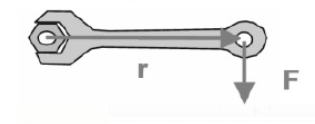
\includegraphics[scale=0.5]{tuerca.png}
\end{figure}

\begin{enumalf}
\item $0,01\ \si{N}$
\item $0,1\ \si{N}$
\item $1\ \si{N}$
\item $10\ \si{N}$
\item $100\ \si{N}$
\end{enumalf}

\item Una persona cierra una puerta de $1\ \si{m}$ de ancho, aplicando una fuerza perpendicular a la puerta de $40\ \si{N}$ a $90\ \si{cm}$ de su eje de rotación. El torque aplicado es:

\begin{enumalf}
\item $3600\ \si{N.m}$
\item $360\ \si{N.m}$
\item $40\ \si{N.m}$
\item $36\ \si{N.m}$
\item $4\ \si{N.m}$
\end{enumalf}

\pagebreak

\item Camila y Daniel están sentados en un balancín homogéneo, como en la figura siguiente donde $A$ representa a Camila y $B$ representa a Daniel. Camila está a $x$ metros del centro, y Daniel está a $y$ metros del centro. A pesar de que Camila y Daniel no pesan lo mismo, el balancín está equilibrado. Esto puede deberse a que

\begin{figure}[h]
\centering
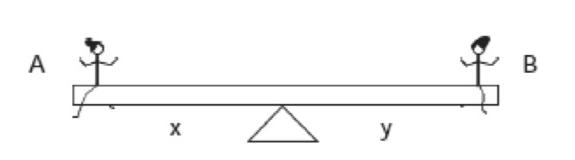
\includegraphics[scale=0.5]{balancin.png}

\end{figure}

\begin{enumalf}
\item el torque aplicado por Camila y el aplicado por Daniel respecto del pivote, es nulo.
\item falta conocer los valores de $x$ e $y$.
\item Camila y Daniel aplican fuerzas de igual magnitud sobre el balancín.
\item el torque neto, respecto del pivote, es nulo en el sistema.
\item el peso que aplica Camila sobre el balancín es menor que el que aplica Daniel.
\end{enumalf}

\item Una moneda que se hace rodar por una mesa puede mantenerse rotando en el mismo plano mientras avanza, mientras que cuando su rapidez angular es muy baja, su movimiento se hace errático hasta que cae y queda en reposo. ¿Usando qué principio se puede explicar que la moneda conserve su plano de rotación?

\begin{enumalf}
\item conservación del momento angular.
\item conservación de la energía.
\item conservación del momento de inercia. 
\item conservación del Torque.
\item Ninguna de las anteriores
\end{enumalf}

\item Dos niñas, Alfa y Beta, empujan una puerta ejerciendo una fuerza perpendicular a la puerta. La puerta puede girar libremente en torno al eje indicado. Si las niñas presionan la puerta y ésta se mantiene inmóvil, podemos afirmar que

\begin{figure}[h]
\centering
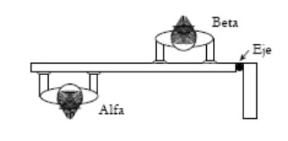
\includegraphics[scale=0.5]{alfabeta.png}
\end{figure}

\begin{enumalf}
\item la magnitud de la fuerza que aplica Alfa sobre la puerta es menor que la que aplica Beta.
\item la magnitud de la fuerza que aplica Alfa sobre la puerta es mayor que la que aplica Beta.
\item Alfa y Beta aplican fuerzas de igual magnitud sobre la puerta.
\item el torque con respecto al eje aplicado por Alfa es nulo.
\item el torque con respecto al eje aplicado por Alfa es mayor que el aplicado por Beta.
\end{enumalf}

\pagebreak

\item Una barra de $2\ \si{m}$ de largo y peso despreciable, está pivotada en un extremo, y en el otro extremo está amarrada a una cuerda que se hace pasar por una polea de $40\ \si{cm}$ de diámetro y de la cual cuelga una masa $A$ de $2\ \si{kg}$. Además de $A$, un cuerpo $B$ de $8\ \si{kg}$ descansa sobre la barra a la izquierda del pivote. Si el sistema está en equilibrio, entonces $B$ está ubicado respecto al punto de apoyo a una distancia de

\begin{figure}[h]
\centering
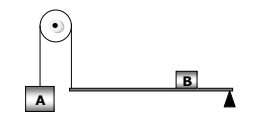
\includegraphics[scale=0.5]{polea1.png}
\end{figure}

\begin{enumalf}
\item $1,5\ \si{m}$
\item $1,0\ \si{m}$
\item $0,5\ \si{m}$
\item $0,4\ \si{m}$
\item $0,2\ \si{m}$
\end{enumalf}

\item Se tiene una barra homogénea de peso $20\ \si{N}$ y largo $L$ en equilibrio rotacional. La barra está pivoteada a una distancia $\frac{L}{4}$ del centro, hacia la izquierda. Si sobre el extremo izquierdo cuelga un cuerpo de masa $5\ \si{kg}$, entonces la masa del cuerpo $M$ que se encuentra en el extremo derecho de la barra es,

\begin{figure}[h]
\centering
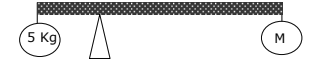
\includegraphics[scale=0.5]{balancin2.png}
\end{figure}

\begin{enumalf}
\item $0,5\ \si{kg}$
\item $1\ \si{kg}$
\item $2\ \si{kg}$
\item $5\ \si{kg}$
\item $10\ \si{kg}$
\end{enumalf}

\item Respecto a la situación de la figura, se hacen las siguientes aseveraciones:

\begin{figure}[h]
\centering
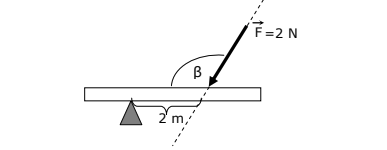
\includegraphics[scale=0.5]{ang.png}
\end{figure}

\begin{enumroman}
\item Si el ángulo $\beta$ aumenta, entonces el torque aumenta.
\item Si el ángulo $\beta$ es \ang{180}, entonces el torque es nulo.
\item No importa el valor que tome el ángulo $\beta$ ya que la magnitud del torque siempre será $4\ \si{N.m}$.
\end{enumroman}

\begin{enumalf}
\item Sólo I
\item Sólo II
\item Sólo III
\item Sólo I y III
\item I, II y III
\end{enumalf}

\item El sistema mostrado en la figura está en equilibrio, en ella también se muestran las distancias al punto de apoyo. Los pesos de las poleas y de la palanca, así como las fuerzas de fricción son despreciables. ¿Cuál es el módulo de la fuerza $\vec{P}$?

\begin{figure}[h]
\centering
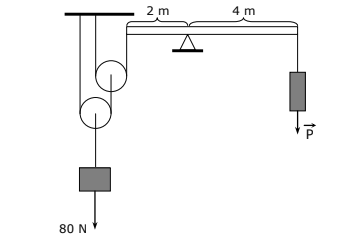
\includegraphics[scale=0.5]{poleas.png}
\end{figure}

\begin{enumalf}
\item $80\ \si{N}$
\item $40\ \si{N}$
\item $20\ \si{N}$
\item $10\ \si{N}$
\item $5\ \si{N}$
\end{enumalf}

Para que una persona pueda mantener el sistema de poleas de la figura en equilibrio, debe ejercer una fuerza vertical de magnitud,

\begin{figure}[h]
\centering
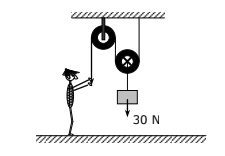
\includegraphics[scale=0.5]{personapolea.png}
\end{figure}

\begin{enumalf}
\item $300\ \si{N}$
\item $150\ \si{N}$
\item $30\ \si{N}$
\item $15\ \si{N}$
\item $7,5\ \si{N}$
\end{enumalf}

\pagebreak

\item Una barra horizontal está apoyada en el extremo izquierdo sobre la cabeza de una persona, y en el extremo derecho sobre un mueble. La barra es homogénea, mide $2\ \si{m}$ de largo y pesa $6\ \si{kg}$. Considerando los torques respecto al extremo derecho de la barra, la fuerza que hace la cabeza de la persona sobre la barra es

\begin{figure}[h]
\centering
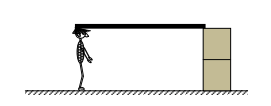
\includegraphics[scale=0.5]{personatorque.png}
\end{figure}

\begin{enumalf}
\item $120\ \si{N}$
\item $60\ \si{N}$
\item $45\ \si{N}$
\item $30\ \si{N}$
\item $20\ \si{N}$
\end{enumalf}

\end{enumerate}

\pagebreak
\begin{center}
\begin{tabular}{|c|c|c|c|c|}
\hline
 1 & 2 & 3 & 4 & 5 \\ \hline
 B & E & A & E & D \\ \hline
 6 & 7 & 8 & 9 & 10 \\ \hline
 D & A & B & C & B \\ \hline
 11 & 12 & 13 & 14 & 15 \\ \hline
 B & D & D & D & / \\ \hline
\end{tabular}
\end{center}


\end{document}